\documentclass{beamer}


\title{Tallahassee Crime Map}
\author{Munawar Ali, Çağatay Ayhan, Ece Karaçam, Abdullah Malik, and Mao Nishino}

\date{\today}

\begin{document}

\begin{frame}
    \titlepage
\end{frame}

\begin{frame}
    \frametitle{Outline}
    \tableofcontents
\end{frame}

%%% Keep the hourly bar-chart
%% add the location bar-chart

\section{Introduction}
\begin{frame}
    \frametitle{Introduction}
    Write two goals of the project: 1) to create a crime map of Tallahassee, and 2) to analyze the crime data using traditional machine learning techniques.
\end{frame}

\section{Data Collection and Processing}
\begin{frame}
    \frametitle{TOPS Data Collection}
    Write a brief description about how we collected the data from TOPS
\end{frame}

\begin{frame}
    \frametitle{Data Processing}
    Write a short description about how we create our map dataset
\end{frame}

%%%%%%%%%%%%%%%%%%%%%%%%%%% SPATIAL ANALYSIS BEGIN %%%%%%%%%%%%%%%%%%%%%

\begin{frame}
    \frametitle{Categorical Analysis}
    \begin{minipage}[c]{0.65\textwidth}
        \begin{figure}
            \centering
            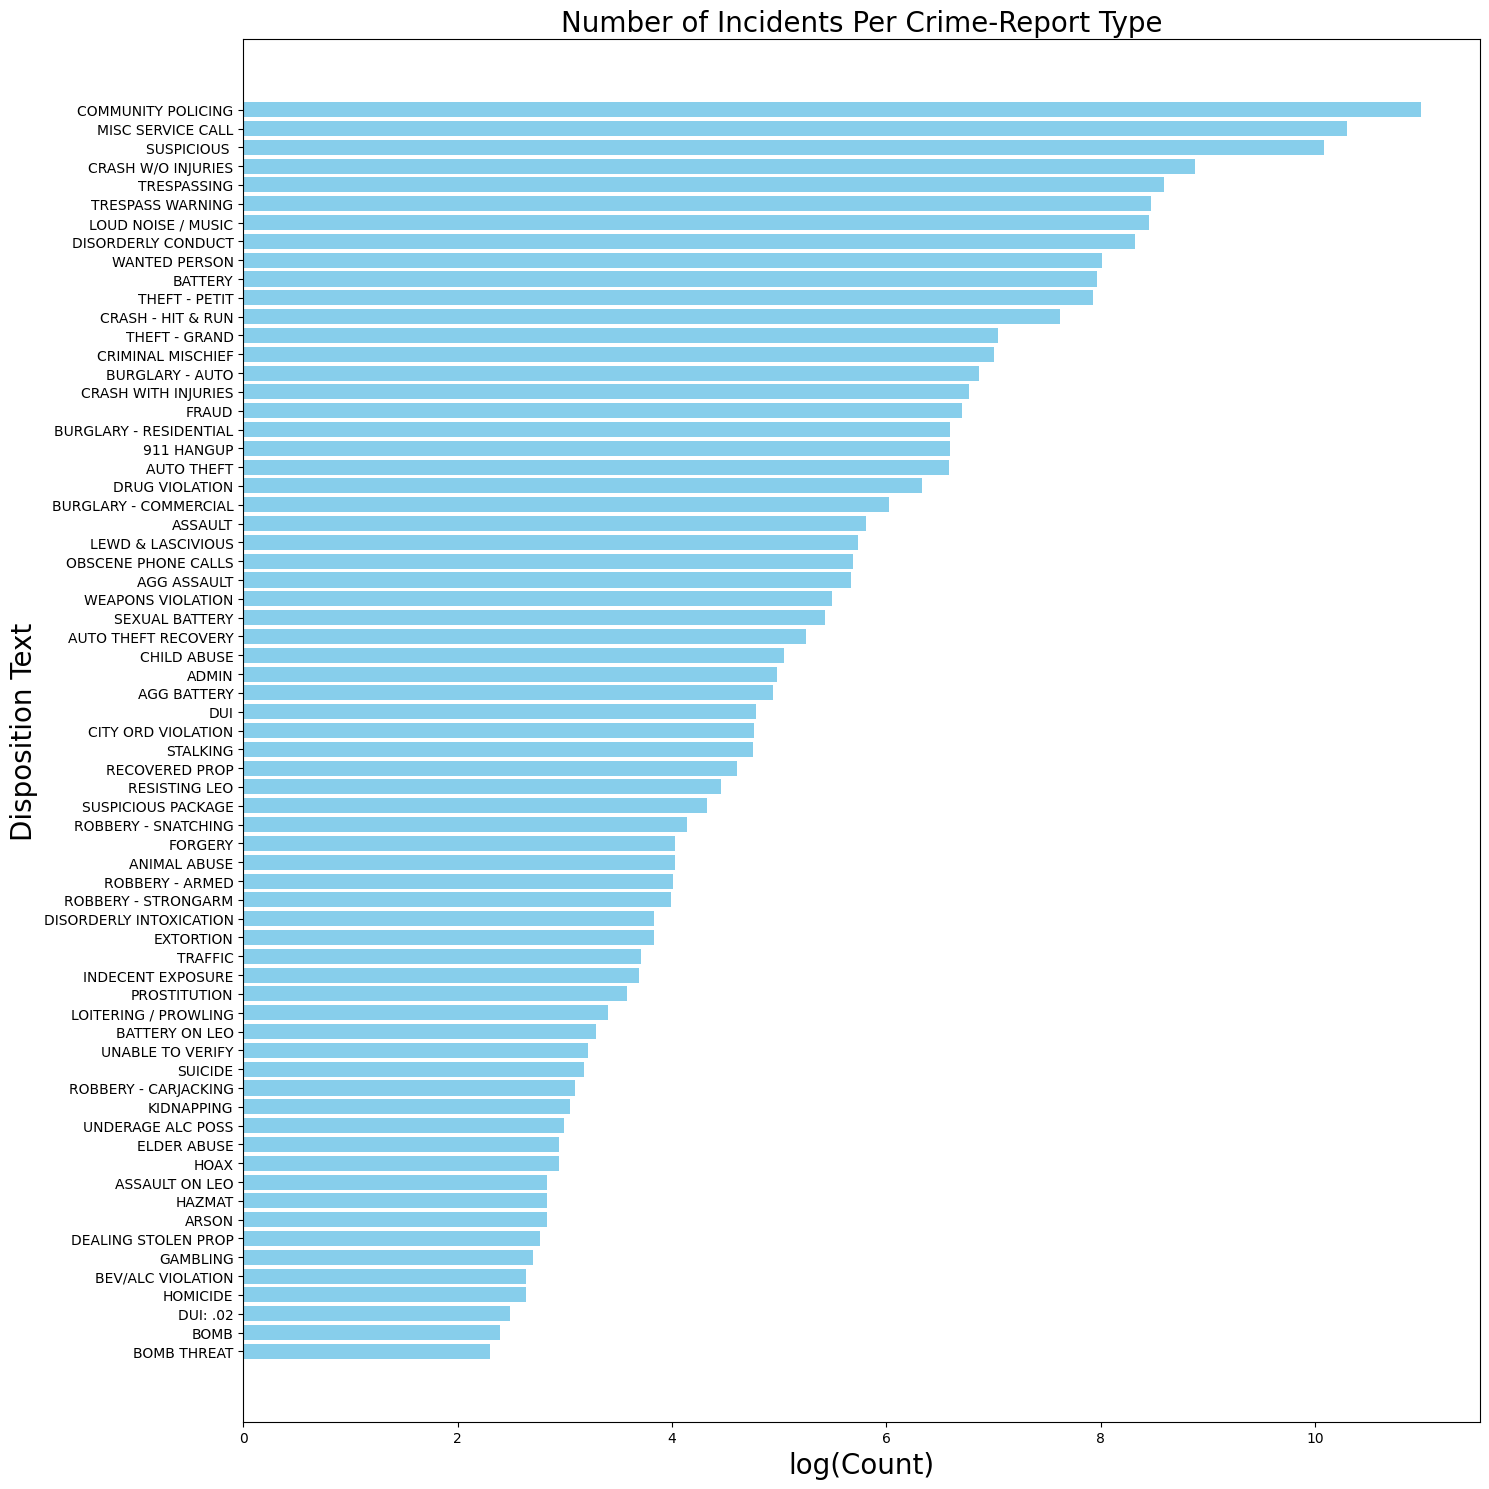
\includegraphics[width=\linewidth]{Figures/Number of Incidents Per Crime-Report Type.png}
            \caption{A bar chart for each type of crime report.}
        \end{figure}
    \end{minipage}\hfill
    \begin{minipage}[c]{0.3\textwidth}
        {\scriptsize % Smaller text to fit more content
        \begin{itemize}
            \item The values on the $x$-axis correspond to the log of the actual count for visual purposes.
            \item On the $y$-axis all different types of crime reports are listed.
            \item There are 67 types of reports.
            \item We will filter out some from our analysis. For example, community policing occurs most often and it is not of interest for our purposes.
        \end{itemize}
        }
    \end{minipage}
\end{frame}








%%%%%%%%%%%%%%%%%%%%%%%%%%% SPATIAL ANALYSIS END %%%%%%%%%%%%%%%%%%%%%%%


%%%%%%%%%%%%%%%%%%%%%%%%%%% TEMPORAL ANALYSIS BEGIN%%%%%%%%%%%%%%%%%
\section{Experimental Data Analysis}
\begin{frame}
    \frametitle{Temporal Analysis}
    % Put figures about temporal trends in crime data (per semester, per month, per day, per hour, etc.)
    \begin{minipage}[c]{0.7\textwidth}
        \begin{figure}
            \centering
            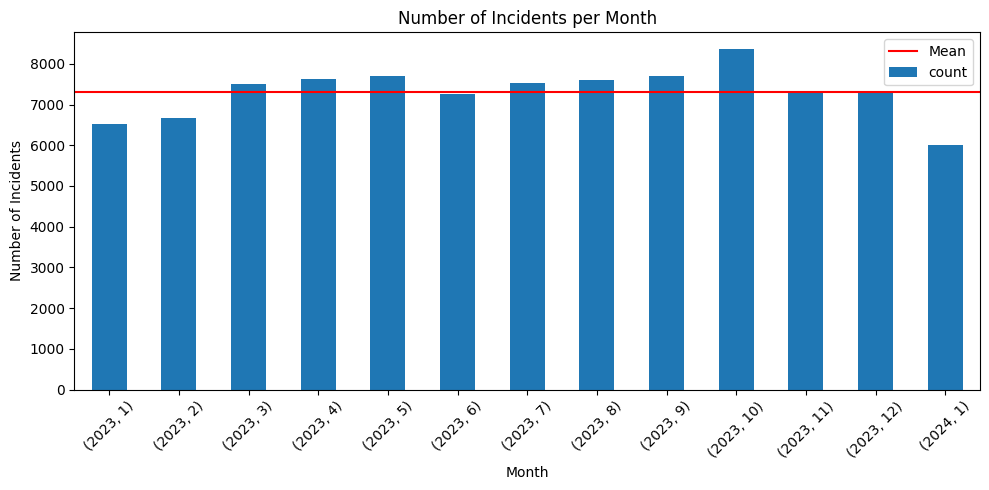
\includegraphics[width=\linewidth]{Figures/Number of Incidents Per Month.png}
            \caption{Crime Distribution Per Month}
        \end{figure}
    \end{minipage}\hfill
    \begin{minipage}[c]{0.3\textwidth}
        {\scriptsize % Smaller text to fit more content
        \begin{itemize}
            \item Average \# of reported crimes per month is $7311$.
            \item Data includes all of 2023 and the first month of 2024.
        \end{itemize}
        }
    \end{minipage}

\end{frame}

%%%%%%%%%%%%%%%%%%%%%%%%%%% Temporal Analysis Page 2 %%%%%%
\begin{frame}
    \frametitle{Temporal Analysis}
    % Put figures about temporal trends in crime data (per semester, per month, per day, per hour, etc.)
    \begin{minipage}[c]{0.7\textwidth}
        \begin{figure}
            \centering
            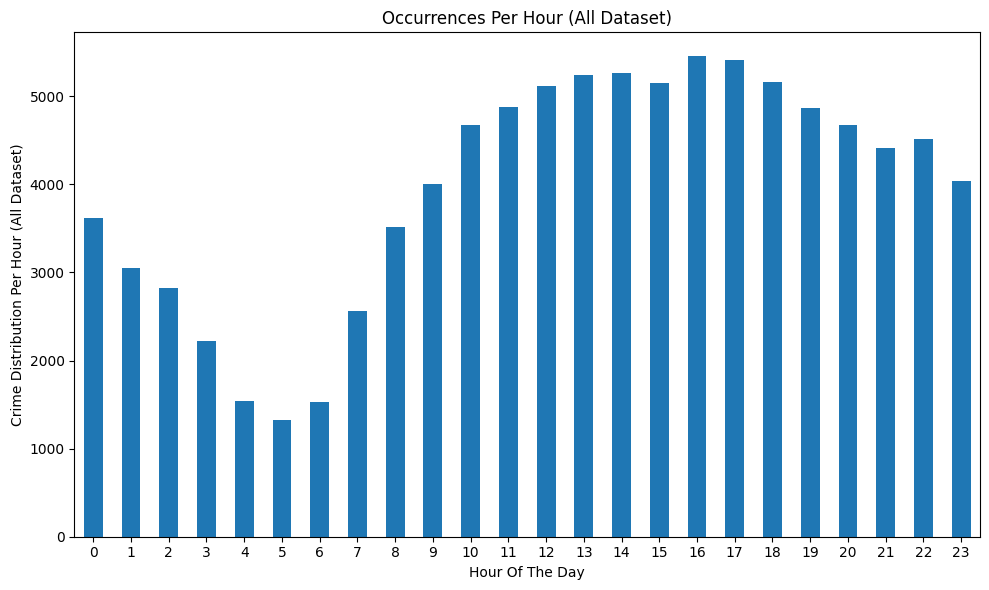
\includegraphics[width=\linewidth]{Figures/Crime Distribution Per Hour (All Dataset).png}
            \caption{Crime Distribution Per Hour -- All 2023}
        \end{figure}
    \end{minipage}\hfill
    \begin{minipage}[c]{0.3\textwidth}
        {\scriptsize % Smaller text to fit more content
        \begin{itemize}
            \item Hourly analysis of the data reveals a fluctuating trend with peak hours.
            \item Data includes all of 2023.
        \end{itemize}
        }
    \end{minipage}

\end{frame}

%%%%%%%%%%%%%%%%%%%%%%%%%%% Temporal Analysis Page 3 %%%%%%

\begin{frame}
    \frametitle{Temporal Analysis}
    % Put figures about temporal trends in crime data (per semester, per month, per day, per hour, etc.)
        \begin{figure}
            \flushleft
            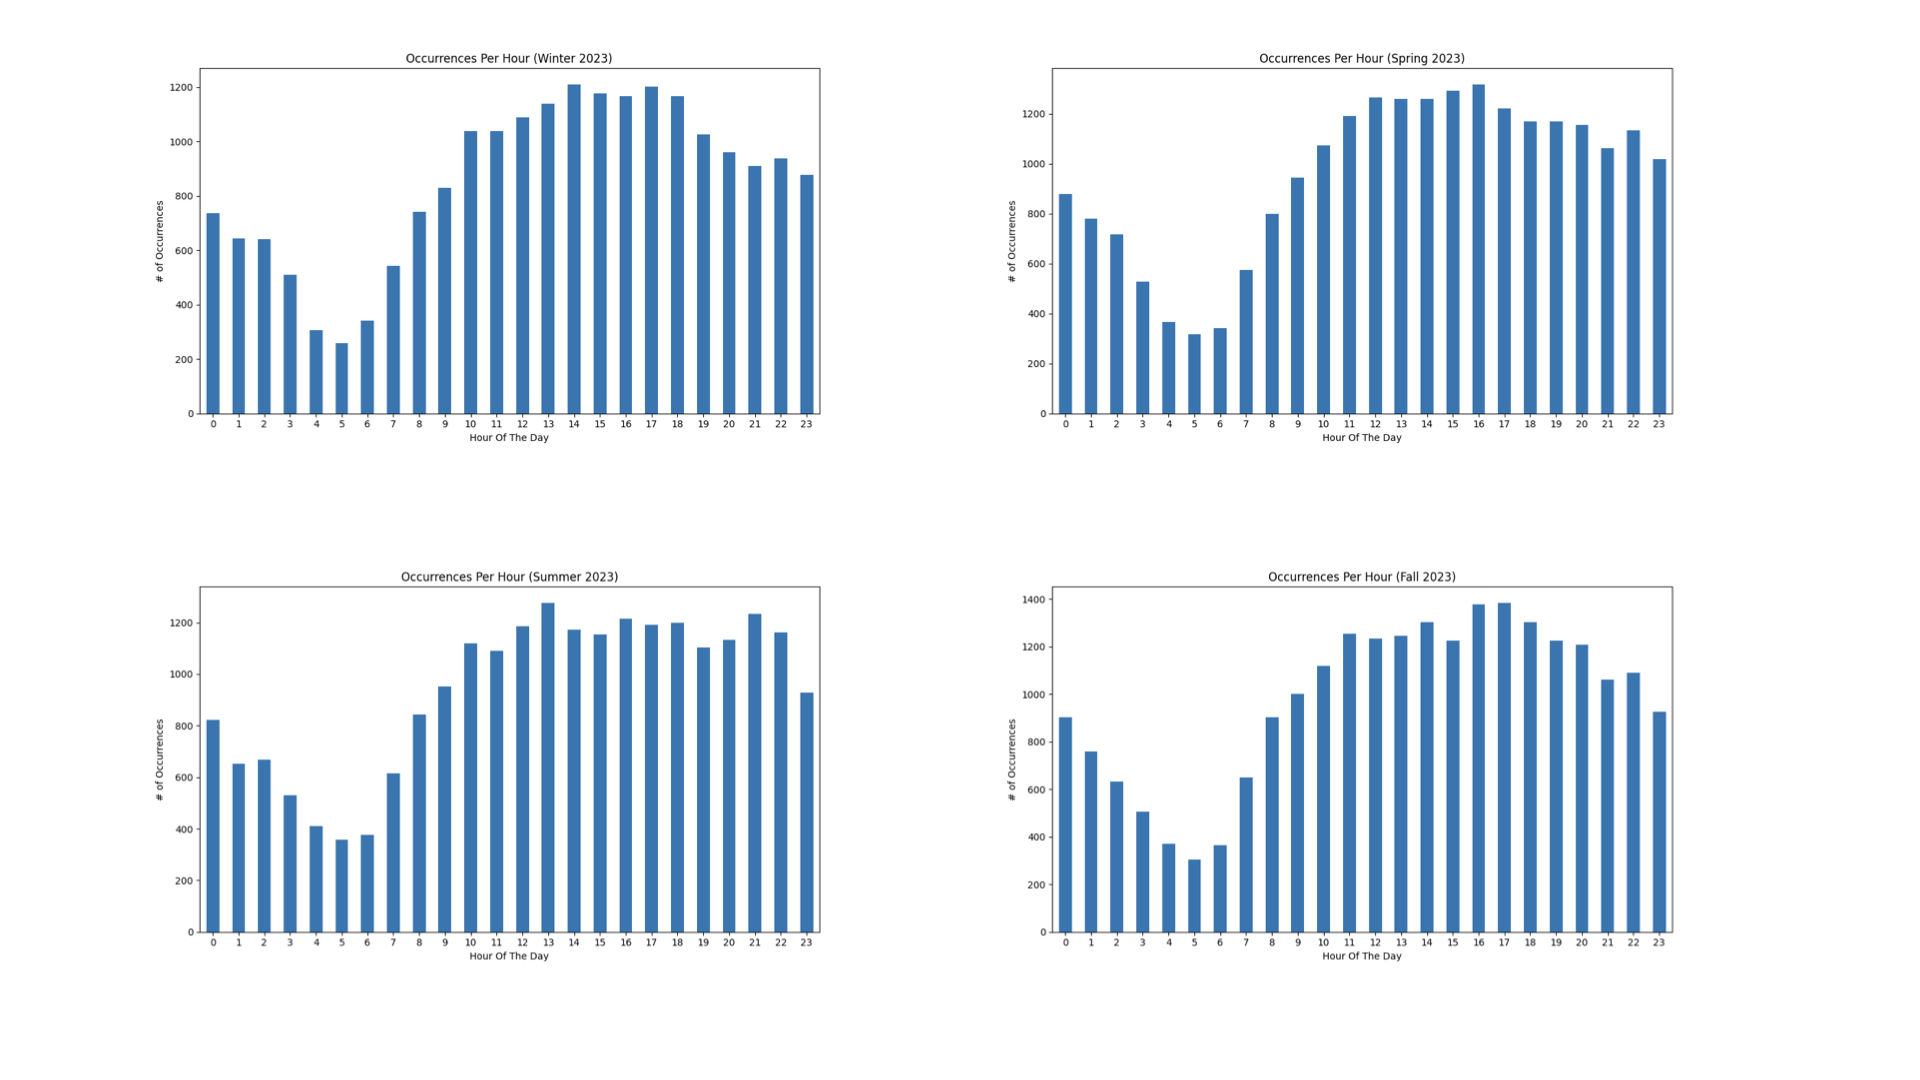
\includegraphics[width=1\linewidth]{Figures/OccurencesPerSeason.001.jpeg}
        \end{figure}
        {\scriptsize % Smaller text to fit more content
        \begin{itemize}
            \item  Hourly crime distribution using portions of the data.
            \item  Same trend across different seasons of the year 2023.
        \end{itemize}
        }
    

\end{frame}

%%%%%%%%%%%%%%%%%%%%%%%%%%% Temporal Analysis Page 4 %%%%%%

\begin{frame}
    \frametitle{Temporal Analysis}
    % Put figures about temporal trends in crime data (per semester, per month, per day, per hour, etc.)
        \begin{figure}
            \flushleft
            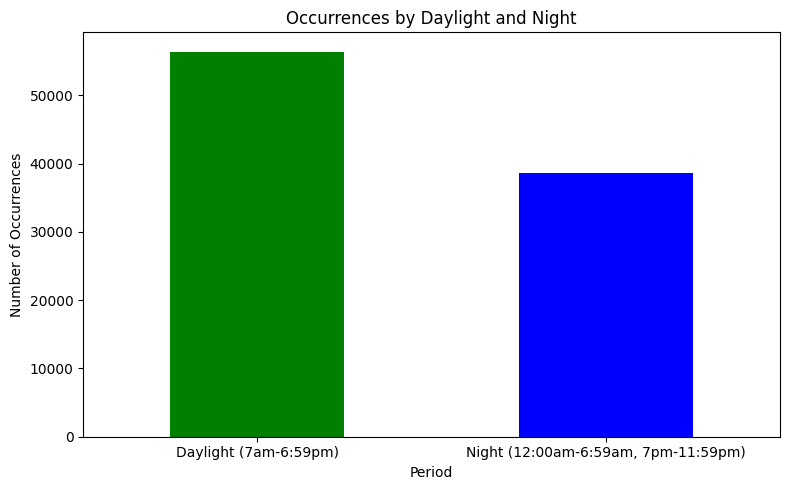
\includegraphics[width=1\linewidth]{Figures/Daylight_and_Night.png}
        \end{figure}
        {\scriptsize % Smaller text to fit more content
        \begin{itemize}
            \item  Daylight vs no daylight. When is an incident more likely to occur?
        \end{itemize}
        }
\end{frame}




%%%%%%%%%%%%%%%%%%%%%%%%%%% Temporal Analysis Page 5 %%%%%%

\begin{frame}
    \frametitle{Temporal Analysis}
    % Put figures about temporal trends in crime data (per semester, per month, per day, per hour, etc.)
        \begin{figure}
            \flushleft
            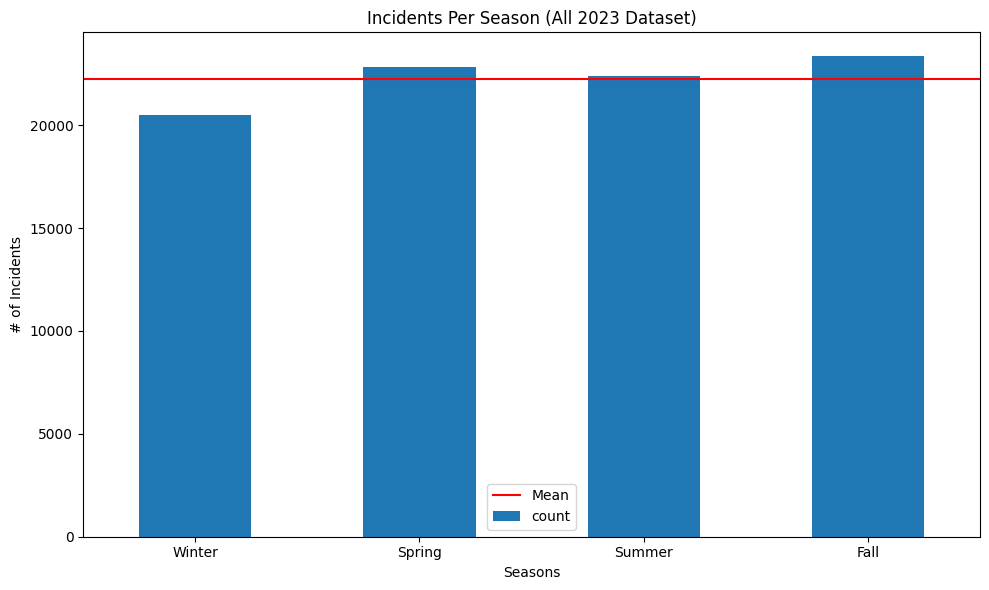
\includegraphics[width=1\linewidth]{Figures/Incidents Per Season (All 2023 Dataset).png}
        \end{figure}
        {\scriptsize % Smaller text to fit more content
        \begin{itemize}
            \item  Crime-report distribution based on seasons.
        \end{itemize}
        }
\end{frame}


%%%%%%%%%%%%%%%%%%%%%%%%%%% Temporal Analysis Page 6 %%%%%%

\begin{frame}
    \frametitle{Temporal Analysis}
    % Put figures about temporal trends in crime data (per semester, per month, per day, per hour, etc.)
        \begin{figure}
            \flushleft
            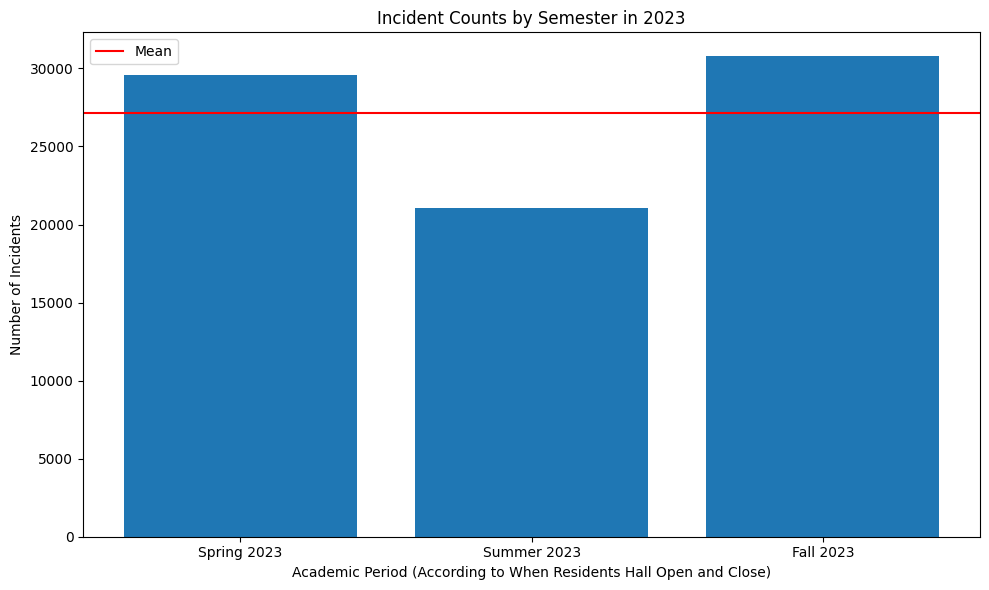
\includegraphics[width=1\linewidth]{Figures/Incident Counts by Semester in 2023.png}
        \end{figure}
        {\scriptsize % Smaller text to fit more content
        \begin{itemize}
            \item Tallahassee is a college town. (FSU \& FAMU \& TCC)
            \item Do students affect the number of crime reports?
        \end{itemize}
        }
\end{frame}


%%%%%%%%%%%%%%%%%%%%%%%%%%% TEMPORAL ANALYSIS END%%%%%%%%%%%%%%%%%%



\section{Crime Heatmap Generation}

\begin{frame}
    \frametitle{pix2pix}
    Brief explanation of GAN and pix2pix
\end{frame}

\begin{frame}
    \frametitle{Results}
    Put the results of the pix2pix model, i.e., the generated heatmap and accuracy
\end{frame}

\begin{frame}
    \frametitle{Improving the city via generated heatmap}
    Edit a geographical map and reduce the crime rate predicted by the model
    Explain how it can be used by city planners
\end{frame}

\section{Conclusion}
\begin{frame}
    \frametitle{Conclusion}
    Summarize the results and a bit of future work (like a web app for the model)
\end{frame}

\end{document}